\chapter{Advanced Future Forms}

\begin{center}
\begin{tabular}{ccc}
\cefrlevel{B1-B2} & \textbf{Study Time:} 3-4 hours & \textbf{Difficulty:} ⭐⭐⭐⭐☆
\end{tabular}
\end{center}

\section{Lesson Objectives}
\begin{tcolorbox}[colback=green!5, colframe=green!40!black, title={📚 By the end of this chapter, you will be able to:}]
\begin{itemize}
    \item [\checkmark] Form and use the Future Continuous for actions in progress
    \item [\checkmark] Form and use the Future Perfect for completed actions
    \item [\checkmark] Form and use the Future Perfect Continuous for duration
    \item [\checkmark] Distinguish between all future forms
    \item [\checkmark] Use timelines to visualize future tenses
\end{itemize}
\end{tcolorbox}

\section{Reading Context}
\begin{readingbox}[title=Dialogue: Planning for the Future]
\textbf{Manager:} This time next week, we\textbf{'ll be presenting} the project to the board.\\
\textbf{Emma:} I know. By Friday, I \textbf{will have finished} all the slides.\\
\textbf{Manager:} Perfect. And by the end of the month, we\textbf{'ll have been working} on this for six months!\\
\textbf{Emma:} Yes! At 2pm tomorrow, I\textbf{'ll be meeting} with the design team to finalize everything.\\
\textbf{Manager:} Excellent. I'm confident that by next month, we \textbf{will have completed} the entire project.
\end{readingbox}

\section{Grammar Focus: Future Continuous}

The future continuous describes actions that \textbf{will be in progress} at a specific time in the future.

\begin{grammarbox}[title=Future Continuous Structure]
\textbf{Structure:} Subject + \textbf{will be} + \textbf{verb-ing}

\textbf{Formation:}
\begin{itemize}
    \item \textbf{Affirmative:} I/You/He/She/We/They + \textbf{will be} + verb-ing
    \item \textbf{Negative:} Subject + \textbf{will not (won't) be} + verb-ing
    \item \textbf{Interrogative:} \textbf{Will} + subject + \textbf{be} + verb-ing?
\end{itemize}

\textbf{Examples:}
\begin{itemize}
    \item This time tomorrow, I\textbf{'ll be flying} to Paris. \trans{Estaré volando}
    \item At 8pm tonight, they\textbf{'ll be having} dinner. \trans{Estarán cenando}
    \item \textbf{Will} you \textbf{be working} late tomorrow? \trans{¿Estarás trabajando?}
    \item I \textbf{won't be sleeping} at midnight. \trans{No estaré durmiendo}
\end{itemize}
\end{grammarbox}

\subsection{When to Use Future Continuous}

\begin{vocabbox}[title=Use Future Continuous for:]
\textbf{1. Actions in progress at a specific future time:}
\begin{itemize}
    \item At 3pm tomorrow, I\textbf{'ll be sitting} in a meeting. \trans{Estaré sentado}
    \item This time next year, she\textbf{'ll be studying} at university. \trans{Estará estudiando}
\end{itemize}

\textbf{2. Future actions that will happen in the normal course of events:}
\begin{itemize}
    \item Don't call at 7pm - we\textbf{'ll be eating} dinner. \trans{Estaremos cenando}
    \item I\textbf{'ll be seeing} Tom tomorrow, so I can give him the message. \trans{Veré a Tom}
\end{itemize}

\textbf{3. Polite inquiries about plans:}
\begin{itemize}
    \item \textbf{Will} you \textbf{be using} the car tomorrow? \trans{¿Vas a usar el coche?}
    \item \textbf{Will} you \textbf{be going} to the shop? \trans{¿Vas a ir a la tienda?}
\end{itemize}
\end{vocabbox}

\section{Grammar Focus: Future Perfect}

The future perfect describes actions that \textbf{will be completed} before a specific point in the future.

\begin{grammarbox}[title=Future Perfect Structure]
\textbf{Structure:} Subject + \textbf{will have} + \textbf{past participle (V3)}

\textbf{Formation:}
\begin{itemize}
    \item \textbf{Affirmative:} Subject + \textbf{will have} + V3
    \item \textbf{Negative:} Subject + \textbf{will not (won't) have} + V3
    \item \textbf{Interrogative:} \textbf{Will} + subject + \textbf{have} + V3?
\end{itemize}

\textbf{Examples:}
\begin{itemize}
    \item By next year, I \textbf{will have completed} my degree. \trans{Habré completado}
    \item By 6pm, she \textbf{will have finished} work. \trans{Habrá terminado}
    \item \textbf{Will} you \textbf{have left} by then? \trans{¿Te habrás ido?}
    \item They \textbf{won't have arrived} yet. \trans{No habrán llegado}
\end{itemize}
\end{grammarbox}

\subsection{When to Use Future Perfect}

\begin{vocabbox}[title=Use Future Perfect for:]
\textbf{1. Actions completed before a future time:}
\begin{itemize}
    \item \textbf{By} Friday, I \textbf{will have finished} the report. \trans{Para el viernes, habré terminado}
    \item \textbf{By} 2030, they \textbf{will have built} 1000 houses. \trans{Para 2030, habrán construido}
\end{itemize}

\textbf{2. To look back from a future point:}
\begin{itemize}
    \item Next week, I \textbf{will have been} here for 5 years. \trans{Habré estado}
    \item In June, we \textbf{will have known} each other for 10 years. \trans{Nos habremos conocido}
\end{itemize}

\textbf{Common with:} by (time), by the time, before, when
\end{vocabbox}

\section{Grammar Focus: Future Perfect Continuous}

The future perfect continuous emphasizes the \textbf{duration} of an activity up to a point in the future.

\begin{grammarbox}[title=Future Perfect Continuous Structure]
\textbf{Structure:} Subject + \textbf{will have been} + \textbf{verb-ing}

\textbf{Formation:}
\begin{itemize}
    \item \textbf{Affirmative:} Subject + \textbf{will have been} + verb-ing
    \item \textbf{Negative:} Subject + \textbf{will not have been} + verb-ing
    \item \textbf{Interrogative:} \textbf{Will} + subject + \textbf{have been} + verb-ing?
\end{itemize}

\textbf{Examples:}
\begin{itemize}
    \item By noon, they \textbf{will have been working} for 5 hours. \trans{Habrán estado trabajando}
    \item In May, I\textbf{'ll have been living} here for 2 years. \trans{Habré estado viviendo}
    \item \textbf{Will} you \textbf{have been waiting} long? \trans{¿Habrás estado esperando?}
\end{itemize}
\end{grammarbox}

\subsection{When to Use Future Perfect Continuous}

\begin{vocabbox}[title=Use Future Perfect Continuous for:]
\textbf{1. Duration up to a future point:}
\begin{itemize}
    \item \textbf{By} next month, I\textbf{'ll have been studying} English \textbf{for} 3 years.
    \item \textbf{By} 6pm, she\textbf{'ll have been working} \textbf{for} 10 hours straight.
\end{itemize}

\textbf{Common with:} for (duration), by (time point), how long
\end{vocabbox}

\section{Comparing Future Continuous, Future Perfect, and Future Perfect Continuous}

\begin{table}[h]
\centering
\small
\begin{tabular}{|l|p{3.5cm}|p{4cm}|}
\hline
\textbf{Form} & \textbf{Use} & \textbf{Example} \\
\hline
\textbf{Future Continuous} & Action in progress at specific time & At 8pm, I'll \textbf{be eating}. \\
\hline
\textbf{Future Perfect} & Action completed before future point & By 8pm, I'll \textbf{have eaten}. \\
\hline
\textbf{Future Perfect Continuous} & Duration up to future point & By 8pm, I'll \textbf{have been eating} for 2 hours. \\
\hline
\end{tabular}
\caption{Advanced future forms comparison}
\end{table}

\section{Visual Timelines}

\subsection{Timeline 1: Future Simple vs Future Continuous}

\begin{figure}[H]
    \centering
    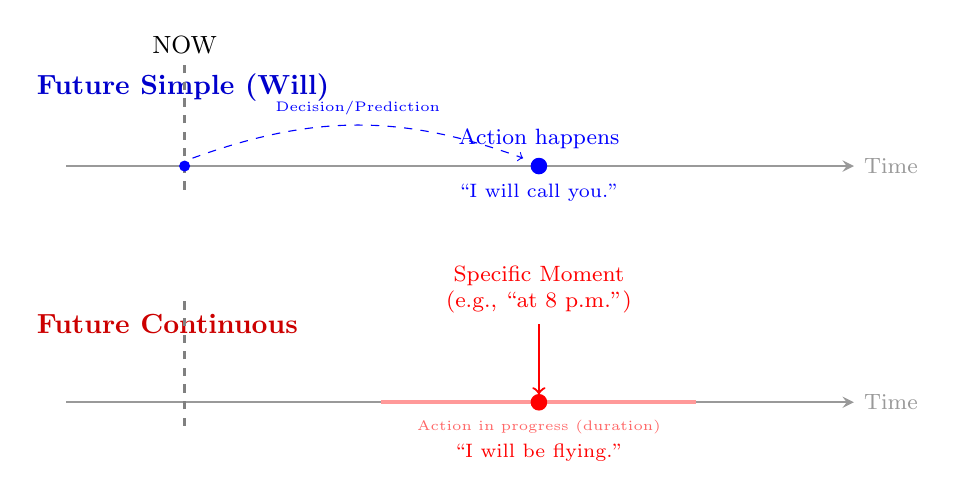
\begin{tikzpicture}[scale=1.0]
        % Common styles
        \tikzstyle{axis}=[->, thick, >=stealth, gray!80]
        \tikzstyle{nowline}=[dashed, thick, gray]
        
        % --- Timeline 1: Future Simple ---
        \node[anchor=west, blue!80!black, font=\bfseries] at (-0.5, 2.5) {Future Simple (Will)};
        \draw[axis] (0, 1.5) -- (10, 1.5) node[right, font=\footnotesize] {Time};
        
        % NOW marker (top)
        \draw[nowline] (1.5, 1.2) -- (1.5, 2.8);
        \node[above, font=\bfseries, font=\small] at (1.5, 2.8) {NOW};
        
        % Event
        \fill[blue] (6, 1.5) circle (3pt);
        \node[above, blue, font=\footnotesize] at (6, 1.6) {Action happens};
        \node[below, blue, font=\scriptsize, align=center] at (6, 1.4) {``I will call you.''};
        
        % Decision arrow
        \draw[->, blue, dashed, bend left=20] (1.6, 1.6) to node[midway, above, font=\tiny] {Decision/Prediction} (5.8, 1.6);
        \fill[blue] (1.5, 1.5) circle (2pt);

        % --- Timeline 2: Future Continuous ---
        \node[anchor=west, red!80!black, font=\bfseries] at (-0.5, -0.5) {Future Continuous};
        \draw[axis] (0, -1.5) -- (10, -1.5) node[right, font=\footnotesize] {Time};
        
        % NOW marker (bottom)
        \draw[nowline] (1.5, -1.8) -- (1.5, -0.2);
        
        % Duration
        \draw[ultra thick, red!40] (4, -1.5) -- (8, -1.5);
        \node[below, red!60, font=\tiny] at (6, -1.6) {Action in progress (duration)};
        
        % Specific moment
        \fill[red] (6, -1.5) circle (3pt);
        \draw[<-, red, thick] (6, -1.4) -- (6, -0.5) node[above, font=\footnotesize, align=center] {Specific Moment\\(e.g., ``at 8 p.m.'')};
        \node[below, red, font=\scriptsize, align=center] at (6, -1.9) {``I will be flying.''};

    \end{tikzpicture}
    \caption{Visual Comparison: Future Simple vs. Future Continuous}
    \label{fig:future_simple_vs_continuous}
\end{figure}

\subsection{Timeline 2: Future Perfect vs Future Perfect Continuous}

\begin{figure}[H]
    \centering
    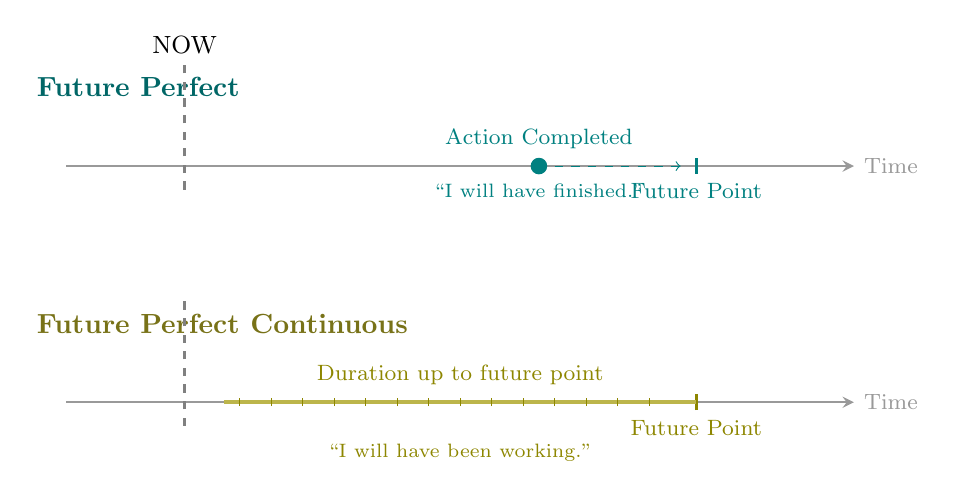
\begin{tikzpicture}[scale=1.0]
        % Common styles
        \tikzstyle{axis}=[->, thick, >=stealth, gray!80]
        \tikzstyle{nowline}=[dashed, thick, gray]
        
        % --- Timeline 1: Future Perfect ---
        \node[anchor=west, teal!80!black, font=\bfseries] at (-0.5, 2.5) {Future Perfect};
        \draw[axis] (0, 1.5) -- (10, 1.5) node[right, font=\footnotesize] {Time};
        
        % NOW marker (top)
        \draw[nowline] (1.5, 1.2) -- (1.5, 2.8);
        \node[above, font=\bfseries, font=\small] at (1.5, 2.8) {NOW};
        
        % Future Point
        \draw[thick, teal] (8, 1.4) -- (8, 1.6);
        \node[below, teal, font=\footnotesize] at (8, 1.4) {Future Point};
        
        % Completed Action
        \fill[teal] (6, 1.5) circle (3pt);
        \node[above, teal, font=\footnotesize] at (6, 1.6) {Action Completed};
        \draw[->, teal, dashed] (6.2, 1.5) -- (7.8, 1.5);
        \node[below, teal, font=\scriptsize, align=center] at (6, 1.4) {``I will have finished.''};

        % --- Timeline 2: Future Perfect Continuous ---
        \node[anchor=west, olive!80!black, font=\bfseries] at (-0.5, -0.5) {Future Perfect Continuous};
        \draw[axis] (0, -1.5) -- (10, -1.5) node[right, font=\footnotesize] {Time};
        
        % NOW marker (bottom)
        \draw[nowline] (1.5, -1.8) -- (1.5, -0.2);
        
        % Future Point
        \draw[thick, olive] (8, -1.6) -- (8, -1.4);
        \node[below, olive, font=\footnotesize] at (8, -1.6) {Future Point};
        
        % Duration
        \draw[ultra thick, olive!60] (2, -1.5) -- (8, -1.5);
        \foreach \x in {2.2, 2.6, ..., 7.8} \draw[olive] (\x, -1.55) -- (\x, -1.45);
        
        \node[above, olive, font=\footnotesize] at (5, -1.4) {Duration up to future point};
        \node[below, olive, font=\scriptsize, align=center] at (5, -1.9) {``I will have been working.''};

    \end{tikzpicture}
    \caption{Visual Comparison: Future Perfect vs. Future Perfect Continuous}
    \label{fig:future_perfect_vs_continuous}
\end{figure}

\subsection{Complete Timeline: All Future Forms}

\begin{figure}[H]
    \centering
    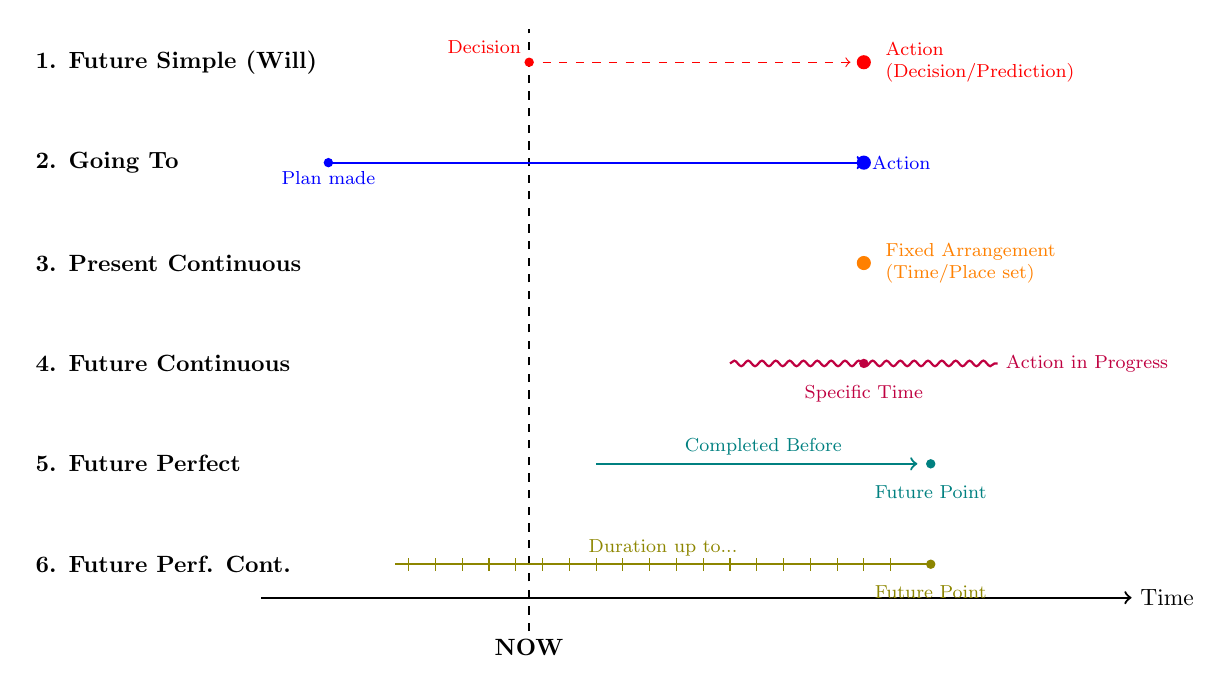
\begin{tikzpicture}[scale=0.85, transform shape]
        % Timeline axis
        \draw[->, thick] (-4,0) -- (9,0) node[right] {Time};
        
        % Now marker
        \draw[thick, dashed] (0, -0.5) -- (0, 8.5);
        \node[below] at (0, -0.5) {\textbf{NOW}};

        % 1. Future Simple (Will)
        \node[anchor=west] at (-7.5, 8) {\textbf{1. Future Simple (Will)}};
        \fill[red] (5, 8) circle (3pt);
        \node[right, red, align=left, font=\footnotesize] at (5.2, 8) {Action\\(Decision/Prediction)};
        \draw[->, red, dashed] (0.2, 8) -- (4.8, 8);
        \fill[red] (0, 8) circle (2pt) node[above left, font=\footnotesize] {Decision};

        % 2. Going To
        \node[anchor=west] at (-7.5, 6.5) {\textbf{2. Going To}};
        \draw[blue, thick, ->] (-3, 6.5) -- (5, 6.5);
        \fill[blue] (-3, 6.5) circle (2pt) node[below, font=\footnotesize] {Plan made};
        \fill[blue] (5, 6.5) circle (3pt) node[right, font=\footnotesize] {Action};

        % 3. Present Continuous
        \node[anchor=west] at (-7.5, 5) {\textbf{3. Present Continuous}};
        \fill[orange] (5, 5) circle (3pt);
        \node[right, orange, align=left, font=\footnotesize] at (5.2, 5) {Fixed Arrangement\\(Time/Place set)};

        % 4. Future Continuous
        \node[anchor=west] at (-7.5, 3.5) {\textbf{4. Future Continuous}};
        \draw[decorate, decoration={snake, amplitude=1pt, segment length=5pt}, thick, purple] (3, 3.5) -- (7, 3.5);
        \fill[purple] (5, 3.5) circle (2pt);
        \node[below, purple, font=\footnotesize] at (5, 3.3) {Specific Time};
        \node[right, purple, font=\footnotesize] at (7, 3.5) {Action in Progress};

        % 5. Future Perfect
        \node[anchor=west] at (-7.5, 2) {\textbf{5. Future Perfect}};
        \draw[->, thick, teal] (1, 2) -- (5.8, 2);
        \fill[teal] (6, 2) circle (2pt);
        \node[below, teal, font=\footnotesize] at (6, 1.8) {Future Point};
        \node[above, teal, font=\footnotesize] at (3.5, 2) {Completed Before};

        % 6. Future Perfect Continuous
        \node[anchor=west] at (-7.5, 0.5) {\textbf{6. Future Perf. Cont.}};
        \draw[thick, olive] (-2, 0.5) -- (6, 0.5);
        \foreach \x in {-1.8, -1.4, ..., 5.8} \draw[olive] (\x, 0.4) -- (\x, 0.6);
        \fill[olive] (6, 0.5) circle (2pt);
        \node[below, olive, font=\footnotesize] at (6, 0.3) {Future Point};
        \node[above, olive, font=\footnotesize] at (2, 0.5) {Duration up to...};

    \end{tikzpicture}
    \caption{Complete Overview: All Future Tenses}
    \label{fig:all_future_tenses}
\end{figure}

\section{Common Mistakes to Avoid}

\begin{tcolorbox}[colback=red!5, colframe=red!60!black, title={Typical Errors}]
\begin{tabular}{|p{5cm}|p{5cm}|}
\hline
\textbf{❌ Incorrect} & \textbf{✓ Correct} \\
\hline
I will \textcolor{red}{been} working. & I will \textbf{be} working. \\
\hline
By Friday, I will \textcolor{red}{finish}. & By Friday, I will \textbf{have finished}. \\
\hline
I will have \textcolor{red}{work}. & I will have \textbf{worked}. \\
\hline
I will have been \textcolor{red}{work}. & I will have been \textbf{working}. \\
\hline
By noon, I will \textcolor{red}{be finished} for 3 hours. & By noon, I will \textbf{have been working} for 3 hours. \\
\hline
\end{tabular}
\end{tcolorbox}

\section{Practice Exercises}

\subsection{Exercise 1: Choose the Correct Form}
Complete with Future Continuous, Future Perfect, or Future Perfect Continuous:

\begin{enumerate}
    \item This time tomorrow, I \underline{\hspace{4cm}} (fly) to New York.
    
    \item By next Friday, she \underline{\hspace{4cm}} (finish) the project.
    
    \item At 8pm tonight, they \underline{\hspace{4cm}} (have) dinner.
    
    \item By June, we \underline{\hspace{4cm}} (work) here for 5 years.
    
    \item Don't call at 3pm - I \underline{\hspace{4cm}} (sleep).
    
    \item By the time you arrive, I \underline{\hspace{4cm}} (wait) for 2 hours.
\end{enumerate}

\subsection{Exercise 2: Correct the Mistakes}
Find and correct the errors:

\begin{enumerate}
    \item By tomorrow, I will be finish the report. \underline{\hspace{5cm}}
    
    \item At 6pm, I will have working for 10 hours. \underline{\hspace{5cm}}
    
    \item This time next week, I will been studying. \underline{\hspace{5cm}}
    
    \item By next year, they will have live here for 3 years. \underline{\hspace{5cm}}
\end{enumerate}

\subsection{Exercise 3: Complete the Sentences}
Use the prompts to write sentences:

\begin{enumerate}
    \item (this time / tomorrow / I / sit / on a beach)
    
    \underline{\hspace{10cm}}
    
    \item (by 2030 / scientists / discover / cure for cancer)
    
    \underline{\hspace{10cm}}
    
    \item (by next month / we / work / on this project / for a year)
    
    \underline{\hspace{10cm}}
\end{enumerate}

\subsection{Exercise 4: Timeline Practice}
Draw a timeline and mark where each action happens:

\begin{enumerate}
    \item At 3pm tomorrow, I'll be meeting the client.
    \item By Friday, I'll have completed all the tasks.
    \item By next month, I'll have been working here for 6 months.
\end{enumerate}

\section{Quick Reference Card}

\begin{tcolorbox}[colback=blue!5, colframe=blue!60!black, title={Chapter Summary}]
\textbf{Key Points to Remember:}
\begin{itemize}
    \item \textbf{Future Continuous:} will be + verb-ing (action in progress at specific time)
    \item \textbf{Future Perfect:} will have + V3 (completed before future point)
    \item \textbf{Future Perfect Continuous:} will have been + verb-ing (duration up to future point)
    \item Use \textbf{BY} + time with Future Perfect forms
    \item Use \textbf{AT} + time with Future Continuous
    \item Use \textbf{FOR} + duration with Future Perfect Continuous
\end{itemize}
\end{tcolorbox}

\section{Key Takeaways}
\begin{itemize}
    \item Future Continuous emphasizes that an action will be \textbf{in progress}
    \item Future Perfect emphasizes that an action will be \textbf{completed}
    \item Future Perfect Continuous emphasizes the \textbf{duration} of an action
    \item These forms are less common but important for precise communication
\end{itemize}

\section{Online Practice}
\begin{tcolorbox}[colback=blue!5,colframe=blue!40!black,title=📱 Resources to Practice]
Reinforce what you have learned with these interactive exercises:
\begin{itemize}
    \item \textbf{Future Continuous:} \url{https://www.perfect-english-grammar.com/future-continuous-exercise-1.html}
    \item \textbf{Future Perfect:} \url{https://learnenglish.britishcouncil.org/grammar/intermediate-to-upper-intermediate/future-perfect}
    \item \textbf{All Future Forms:} \url{https://www.englishpage.com/verbpage/futuretenses.html}
    \item \textbf{Interactive Practice:} \url{https://test-english.com/grammar-points/b1/future-continuous-future-perfect/}
\end{itemize}
\end{tcolorbox}
